\chapter{Logic and Sets}
\begchap{B}efore we jump into proofs, we will discuss two fundamental mechanisms of proof: logic and sets. The purpose of a proof is to logically derive a statement from the initial conditions. In order to be able to do so, we need to understand logic. Further, analyzing logic can give rise to new means of proofs. Next, sets are among the most fundamental object of mathematics, and a nice way to begin very small proofs. Further, sets are useful in that they constitute the universal language to define, organize, and reason about mathematical objects. We thus study the two in greater detail before we begin proofs. 
\section{Logic}
Logic is the foundation of a math proof; the whole purpose of a proof is to logically deduce a statement from existing statements. The cornerstone of logic are if-then statements. If $a = 1$ and $b = 2$, then $a + b = 3$. We have some outcome dependent on some initial condition. Now note that there are not always explicit initial conditions like specifying variables. 1+1 = 2 is a logical statement, but there is no "if" clause. Most competition math problems on tests like USA(J)MO, or your country's equivalent, and IMO, will often ask you to prove statements of this form. For example 

\begin{exercise}
Prove for all positive integers $a$, $x$ also a positive integer, $ax > 0$.
\end{exercise}

While this is not necessarily representative of the difficulty at problems at these competitions (the "proof" is very very short using basic logic), it is an illustrative example of an implicit if-then statement. The "if" here was the statement that $a$ and $x$ are positive integers, and the then statement was that $ax > 0$. These form the basis of mathematical logic. Moving from if-then statements, we have five major types of statements. The first, we already covered. The base statement, or the base if-then argument. To keep it general, we will denote this statement \[P \implies Q\]where the right arrow shows "implies", which is essentially an alternate means of showing an if-then statement (equivalent to initial conditions $P$ implying $Q$, just as if $P$ then $Q$). A simple example of an if-then statement is "if it is raining, the grass is wet".

The second type of statement is the negation of the base. Before we talk about the negation, we will define that $\neg P$ means "not $P$".  "Not $P$" may be denoted in various ways across various books and resources, and thus it is not very common notation (though mathematicians usually know what this denotes). However, we will use it to get you accustomed to notation and for shorthand. When you are writing a proof, I advise you to define this notation beforehand as I have done or just write out "not $P$". Then, we define the negation 
\[P \land \neg Q\] 
\noindent where $\land$ means "and". Again, this is another piece of notation used heavily by logicians, those who study basic axioms and logic. This slightly differs from our if then statement; we don't have that clear structure here. Our example becomes "it is raining and the grass is not wet". The negation essentially describes when the base statement is false. The only way our base statement $P \implies Q$ is false was if $P$ did not necessarily mean $Q$. However, $P \implies \neg Q$ is too strong of a statement, since this is an if-then statement that says P implied not Q; "if it is raining, the grass will not be wet". However, that does not necessarily describe the base falsehood of our original statement. If $P \implies Q$, if rain causes the grass to become wet, then we have that all instances of rain wet the grass. Thus, the one example of rain and grass not being wet is enough to prove the falsehood of the original statement, without needing the condition for all instances of rain. To be more precise, let's consider another example. We have the statement 
\[x \geq a \implies f(x) =0\]
\noindent for some function $f$. It is worth noting the implicit extra condition here. The statement claims that for all $x \geq a$, we will have $f(x)=0$. Thus, if this were to not be true, then it suffices to provide one specific value as a counterexample. Say there exists some number $c \geq a$ such that $f(c)=1$. This is enough of a counterexample to prove the original if statement false. Thus, we have an example, where $x=c$, that \[
x \geq a \land f(x) \neq0
\]
\noindent Notice how this is different from the statement $P \implies \neg Q$. This would translate to the following: $x \geq a \implies f(x) \neq 0$. This new statement claims that for all values of $x$ which is greater than or equal to $a$, the function $f(x)$ is not equal to zero. While this shows that the original statement is false, it is too strong of a statement in that we use much more information, requiring $f(x)$ for all $x$ to make this claim, as compared to the one counterexample before. While this serves as basic intuition for why the negation uses an and and not a negation, we will see in the next chapter that the technique of counterexample is a very important method in actually proving statements. 

The third type of statement is a bit more simple; the converse. Given our base statement, the converse is 
\[Q \implies P\]
\noindent "if the grass is wet, it is raining". It is just the other way around from our base statement. There is not significant comment on this statement; it is relatively logical as is.

\begin{exercise}
Can both the original statement and the negation be true simultaneously? Can the original statement and the converse be true simultaneously?
\end{exercise}

It turns out, the second question is actually very important. When both the original statement and the converse are true, we have a bidirectional statement (fourth type)! 
\[P \iff Q\]
\noindent means "$P$ is true if and only if $Q$ is true". Try to logic and deduce why the original and the converse give us this statement. We can also sometimes replace the bidirectional arrow with an "iff", shorthand for "if and only if". These statements are very strong in that they require both "weaker" conditions to be true (statement and converse). However, note that this may not always be true. As we have seen through the example of rain, the statement is not always true just because the original statement is true. This is what gives a bidirectional statement more importance; it simultaneously requires the truth of two statements and thus contains more information.

The fifth type of statement is the contrapositive. We have seen that in most of the previous statements, nothing is implied purely from the base statement. We do not know whether the converse is true or not, nor do we know whether or not it is bidirectional (we know the inverse is not true if our original statement is not true). However, we can deduce using logic that if the original statement is true, then the contrapositive 
\[\neg Q \implies \neg P\] 
\noindent is true. If the grass is not wet, it is not raining. In our hypothetical world, this is true. The only way for the grass to be wet is for it to be raining. However, note that mathematical logic does not always hold in the real world (at-least in the basic form presented here). Let's return to the statement we used in the negation, $x\geq a \implies f(x) = 0$, in my hopes to persuade you to believe in the contrapositive. The contrapositive of this statement is 
\[f(x) \neq 0 \implies x < a \]
\noindent We know this is true from the original statement; the contrapositive is more sensical in the world of mathematics. If the function does not equal zero, then $x$ must be less than $a$; if not and $x$ was instead greater than or equal to $a$, we would have $f(x)=0$, which contradicts the condition of $f(x) \neq 0$, and thus we cannot have $x \geq a$. Once you are (hopefully) convinced of the truth of the contrapositive (try to logic it out yourself!), we can thus make the following claim:
\[(P \implies Q) \iff (\neg Q \implies \neg P)\]
\noindent This is painful and often nonsensical to put into words through our example with the rain. However, this relationships essentially shows that the contrapositive is always true if the original statement is true, and the original statement is true when the contrapositive is true. This is most powerful in that we often construct proofs of the contrapositive of a statement (more in chapter 3) to imply that the original statement itself is true; this technique is often called proof by contrapositive. We thus have two basic methods of proofs. The second method I have yet to mention is called proof by contradiction, which relies on proving that the negation is false. $(P \implies Q) \iff \neg(P \land \neg Q)$. We will see these two types of proof further in chapter 4.

\section{Sets}
The basic element in nearly all proofs are sets. Sets are easy enough to state, but turns out, quite difficult to understand! 

A set is a collection of things. That's it! Here is a few examples of sets:
\begin{itemize}
    \item A set of my favorite fruits: $F = \{ \text{Apple, Banana, Pear}\}$
    \item A set of my favorite numbers: $P = \{ 15, \pi, 196883,  \hbar\}$
    \item A set of all humans on the Earth: 
    \[H = \{ \text{Me, You, Alice, ...}\}\]
    \item A set of random junk: $J = \{ 342.123413, \frac{9}{43}, 3.1415...,$ Shakespeare, $\phi,$ this book, $\{1, 2, 3, ... \}, \\ \{ 15, \pi, 196883, \hbar\}, \mathbb{N}, ... \}$
    \item A set of all \emph{natural numbers}: $\mathbb{N} = \{ 1, 2, 3, ... \}$
    \item A set of sets of my favorite things: 
    
    \noindent $K = \{ \{ \text{Apple, Banana, Pear}\},$
    $\{ 15, \pi, 196883, \hbar\}, ...\}$
    \item An \emph{empty set}: $E = \emptyset$
    \item A \emph{singleton set}: $\{ \text{Bob}\}$
\end{itemize}

\begin{exercise}
    Make some more of your own sets! 
\end{exercise}

We have used a few conventions here. A set is denoted by a collection of things contained within brackets ($\{ \}$). Also note that ellipses ($...$) is used to show that the set contains more elements that I'm not going to fully list out. Notice some key facts: sets can contain sets inside of them, the elements in a set don't need to be the same "type", sets can be empty, and sets can be infinitely large ($\mathbb{N}$). 

I have further included some key sets we will discuss further. While most variable names I chose for my sets are just arbitrary (if you ask mathematicians what is set $J$ they won't tell you it is the set of junk!), one is especially important: $\mathbb{N}$. $\mathbb{N}$ is widely known as the set of natural numbers, starting $1, 2, 3, ...$ and heading off towards infinity. This is a common convention in math; if you ask a mathematician what $\mathbb{N}$ is, they will know. Further, note the empty set, denoted $\{ \}$ or more commonly using the symbol $\emptyset$, is also an important set, though $E$ is a variable name I chose, not a convention. Keep in mind that the empty set \textbf{is not} $\{ 0 \}$. This leads us nicely into our next name: a singleton set. There is no fixed singleton set, like there was a defined $\mathbb{N}$ or $\{ \emptyset \}$; rather, a singleton set can refer to any set with only one element in it. 

Some other important defined sets are: 
\begin{itemize}
    \item $\mathbb{Z} = \{...,  -2, -1, 0,1, 2, ...\}$, the set of integers.
    \item $\mathbb{N}_0 = \{ 0, 1, 2, ... \}$, the set of natural numbers including zero.
    \item $\mathbb{Z}_{\ge 0} = \{ 0, 1, 2, ... \}$, the set of nonnegative integers.
    \item $\mathbb{Q}$, the set of all rational numbers (can be expressed as a fraction, like $\frac{7}{400}$, but not like $\pi$).
    \item $\mathbb{R}$, the set of all real numbers.
    \item $\mathbb{C}$, the set of all complex numbers.
\end{itemize}
Below is a diagram of the relations between these sets. 
\begin{center}
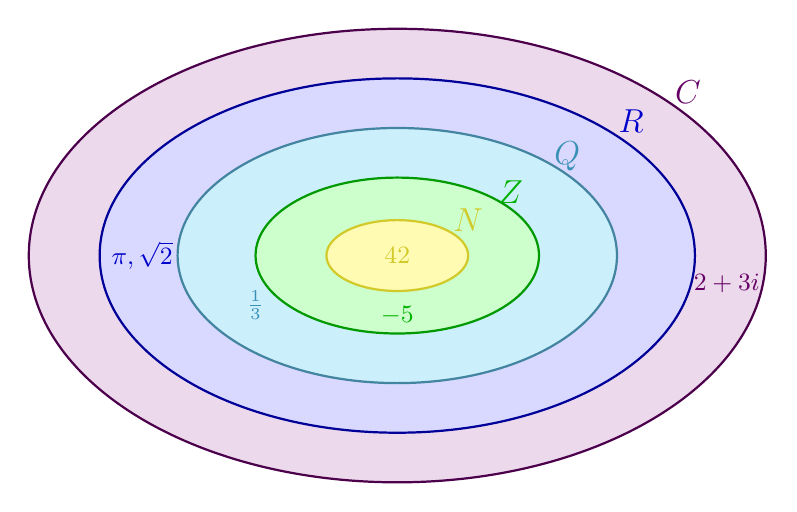
\begin{tikzpicture}[scale=.9]

  % C - outermost
  \fill[violet!15] (0,0) ellipse (5.2cm and 3.2cm);
  \draw[thick, violet!60!black] (0,0) ellipse (5.2cm and 3.2cm);
  \node[violet!80!black, font=\large\bfseries] at (4.1, 2.3) {$\mathbb{C}$};

  % R
  \fill[blue!15] (0,0) ellipse (4.2cm and 2.5cm);
  \draw[thick, blue!60!black] (0,0) ellipse (4.2cm and 2.5cm);
  \node[blue!80!black, font=\large\bfseries] at (3.3, 1.9) {$\mathbb{R}$};

  % Q
  \fill[cyan!20] (0,0) ellipse (3.1cm and 1.8cm);
  \draw[thick, cyan!60!black] (0,0) ellipse (3.1cm and 1.8cm);
  \node[cyan!70!black, font=\large\bfseries] at (2.4, 1.4) {$\mathbb{Q}$};

  % Z
  \fill[green!20] (0,0) ellipse (2.0cm and 1.1cm);
  \draw[thick, green!60!black] (0,0) ellipse (2.0cm and 1.1cm);
  \node[green!70!black, font=\large\bfseries] at (1.6, 0.9) {$\mathbb{Z}$};

  % N - innermost
  \fill[yellow!30] (0,0) ellipse (1.0cm and 0.5cm);
  \draw[thick, yellow!80!black] (0,0) ellipse (1.0cm and 0.5cm);
  \node[yellow!80!black, font=\large\bfseries] at (1.0, 0.5) {$\mathbb{N}$};

  % Example elements in each region
  \node[yellow!80!black, font=\small] at (0, 0)  {$42$};
  \node[violet!80!black, font=\small] at (4.65, -0.4)  {$2+3i$};
  \node[blue!80!black,   font=\small] at (-3.6, 0)    {$\pi, \sqrt{2}$};
  \node[cyan!70!black,   font=\small] at (-2.0, -0.7) {$\frac{1}{3}$};
  \node[green!70!black,  font=\small] at (0, -0.85)   {$-5$};

\end{tikzpicture}
\end{center}

To fully understand this, we need to talk about a couple of things. First, subsets. A subset of a set is somewhat self explanatory. To construct a subset, you may choose any number of elements from the set. For example, the set $S = \{\phi, \frac{9}{43}\}$ is a subset of the junk set $J$ I defined earlier. We denote this $S \subset J$. Note that J itself is a subset of J, and so is the empty set: $\emptyset \subset J$.

Next, is cardinality of sets. The cardinality is just the size of a set. The subset $S$ had cardinality 2, while the cardinality of the set of my favorite numbers has cardinality 4. A singleton set has, by definition, cardinality 1, and the empty set has cardinality 0. Notice that subsets of a (finite) set $K$ can only have cardinality less than or equal to the $K$. We may denote the cardinality by putting bars around the set: $|S| = 2$. You may also see it being denoted by $n(S) = 3$. 

Now using this, we can ask a couple of important questions.
\begin{exercise}
    First, what is the relationship between $\mathbb{N}, \mathbb{Z}, \mathbb{Q}, \mathbb{R}, \mathbb{C}$?
\end{exercise}

Inspection of the diagram along with logic will give us the result that they are all subsets of each other, in the specific following order:
\[\mathbb{N} \subset \mathbb{Z} \subset \mathbb{Q} \subset \mathbb{R} \subset \mathbb{C}\]

Notice that, for example, $\mathbb{Z} \subset \mathbb{R}$ is also a true statement, while $\mathbb{R} \subset \mathbb{N}$ is NOT true. The relationship between these sets follows the relation in the diagram, with the smaller sets being contained inside of the larger ones. 

Now this leads us to ask the next, VERY important (and very difficult) question: what are the cardinalities of these sets? 

\begin{exercise}
    Try to think through this; see what you can come up with. Back your ideas with reasoning.
\end{exercise}

It may intuitively seem at first that the cardinalities of each of the sets is infinity, since there are infinitely many elements in each. However, some infinities are more than others. It may seem that there are more integers than natural numbers; after all there are no negative numbers included in the natural numbers but they are included in the integers. Similar situation between integers and rationals (why?). So what do we do?

For now, I will just tell you the answer; the proof is quite complicated (you will glimpse this in the problem set) The solution is that $\mathbb{N}, \mathbb{Z}, \mathbb{Q}$ are all of the same cardinality, $\aleph_0$ $\sim$ $\infty$ (aleph-nought) , while the $\mathbb{R}$ and $\mathbb{C}$ are of cardinality $2^{\aleph_0}$. These are referred to as countably infinite and uncountable infinite, respectively (though it doesn't make sense now, since infinity is by definition uncountable...). Note that $\aleph_0$ is not a number to be used in a common setting, you should choose to use $\infty$ in most cases, but formally, the notation is $\aleph_0$ if you are working in sets or set theory specifically. Note that $|\mathbb{R}| = \infty$ or $|\mathbb{N}| = \infty$ are usually acceptable statements, unless you need the distinction between countable and uncountable infinities or are using the properties of these separate sets and their different sizes to prove a point. However, you SHOULD NOT use both of these statements together, as use of the above statements in conjunction imply both sets are of the same size.

With that brief introduction to sets, let's talk about set operations. First, the Union operator $\cup$. Think of this sort of like an addition operator. Refer to the below image.

\begin{center}
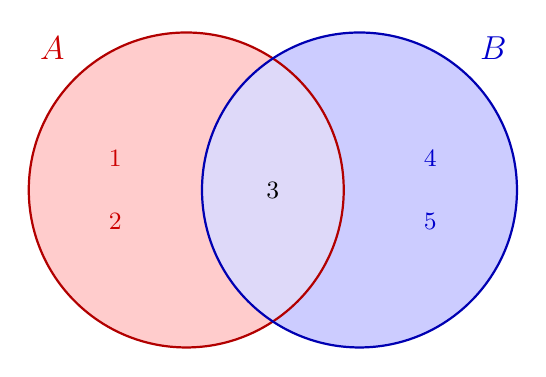
\begin{tikzpicture}[scale=1.0]

  % Two circles
  \def\radius{2.0cm}

  % Fills
  \begin{scope}
    \clip (-1.1, 0) circle (\radius);
    \fill[red!20] (-1.1, 0) circle (\radius);
  \end{scope}
  \begin{scope}
    \clip (1.1, 0) circle (\radius);
    \fill[blue!20] (1.1, 0) circle (\radius);
  \end{scope}

  % Intersection fill
  \begin{scope}
    \clip (-1.1, 0) circle (\radius);
    \clip (1.1, 0) circle (\radius);
    \fill[red!15!blue!15] (-1.1, 0) circle (\radius);
  \end{scope}

  % Outlines
  \draw[thick, red!70!black]  (-1.1, 0) circle (\radius);
  \draw[thick, blue!70!black] ( 1.1, 0) circle (\radius);

  % Set labels
  \node[red!80!black,  font=\large\bfseries] at (-2.8,  1.8) {$A$};
  \node[blue!80!black, font=\large\bfseries] at ( 2.8,  1.8) {$B$};

  % Elements
  \node[red!80!black,  font=\small] at (-2.0,  0.4) {$1$};
  \node[red!80!black,  font=\small] at (-2.0, -0.4) {$2$};
  \node[font=\small]                at ( 0,    0)   {$3$};
  \node[blue!80!black, font=\small] at ( 2.0,  0.4) {$4$};
  \node[blue!80!black, font=\small] at ( 2.0, -0.4) {$5$};

\end{tikzpicture}
\end{center}

For this section, we will define set $A = \{ 1, 2, 3\}$ and set $B = \{ 3, 4, 5\}$. We can use the Venn diagram to answer the question. If we are to take the union of these two sets, it would be \[A \cup B = \{ 1, 2, 3, 4, 5\}\]Notice that 3 is included, but only once (sets cannot have repeat elements!). Now, the second major operator: $\cap$. This is the intersection operator, which is basically the intersection of two sets. In this example, \[A \cap B = \{3\}\]Notice that oftentimes, the intersections of two sets may be the empty set. We call these sets mutually exclusive (for example $\{ 1, 2\}$ and $\{ 3, 4\}$, where $\{ 1, 2\} \cap \{ 3, 4\} = \emptyset$). A couple other useful definitions include the complement of a set denotes $A'$ or $ A^c$. Now, the complement is usually best understood in the context of some universe, or some larger enveloping set. In the above example, we can intuitively define this larger enveloping set to be $\mathbb{N}$, since $A \subset \mathbb{N}$ and $B \subset \mathbb{N}$, so they live in the same "universe". We could have also defined our universe to be $\mathbb{R}$, since is still encompasses $A$ and $B$. We will stick with $\mathbb{N}$ for now, since it is simplest and makes most intuitive sense. However, depending on the situation, either may make sense. In this universe, \[A' = \{4, 5, 6, ...\}\]

Now that we have knowledge of a set and some basic set operations, let us consider a key nontrivial binary operation with sets (other than the union or intersection or complement of those sets). What is the (direct) product of two sets? If we have sets $A$ and $B$
\[
A = \{ 1, 2, 3, 4 , 5\} ~~~~ B = \{0, 6, 7, 8, 9, 10 \}
\]
then what is $A \times B$? 

An element of $A \times B$ is a tuple (or an ordered pair, in this context we can use these terms interchangeably) $(a, b)$ where $a \in A$ and $b \in B$. For example, $(1, 0) \in A \times B$ but $(5, 5) \notin A \times B$. It is a set in which elements are tuples where each element of the tuple is from a specific set. 

Consider the standard x-y plane, that we all know so very well. Each ordered pair is of the form $(x, y)$, hence the name of x-y plane. However, we can also consider this from a different light, which is often the norm in the math community beyond high school. $x \in \mathbb{R}$ and $y \in \mathbb{R}$, which gives us that 
\[
(x, y) \in \mathbb{R} \times \mathbb{R}
\]
This is perfectly valid! We construct a new set which is the direct product of $\mathbb{R}$ with itself, and each tuple $(x, y)$ is from this product since both $x$ and $y$ are each from one of the elements of the product ($\mathbb{R}$). You will see this more commonly denoted as
\[
(x, y) \in \mathbb{R}^2
\]
which makes sense in a way if we treat the exponent simply as a notational shorthand for repeated multiplication (philosophically, this is all the exponent is...). 

In this similar fashion, for example, you may see the set $\mathbb{R}^3$, which simply refers to the set of all points in 3-dimensional space, with tuples oftentimes denoted $(x, y, z)$. Most times, in research, researchers prefer to use vectors instead of tuples for the majority of purposes, so don't stress too much if you stumble upon something like $\vec{v} \in \mathbb{R}^n$! For now, just know that a vector is basically the same thing as a point, where $\vec{v}$ denotes some arbitrary tuple $(x_1, x_2, \ldots, x_n)$.

Also note that this convention is not restricted to $\mathbb{R}$. $\mathbb{Z}^n$ and $\mathbb{C}^n$ are all also perfectly valid and very often used as well. However, keep in mind the key concept of direct product of sets: they produce tuples which each element is from its constituent set.

\begin{exercise}
    Given $|A| = x$ and $|B| = y$, what is $|A \times B|$? How does this compare to $|A \cup B|$ (assuming $A \cap B = \emptyset$)?
\end{exercise}

Now that we have "set multiplication", let us consider "set division". Specifically, given a set $A = \{ 1, 2, 3, \ldots, 20\}$ and $B = \{-10, -9, -8 \ldots, 10 \}$, we will look at the set 
\[
A \setminus B = \{11, 12,13, \ldots, 20 \}
\]
Essentially, $A \setminus B$ is the set of all elements $a \in A$ such that $a \notin B$. 
\begin{center}
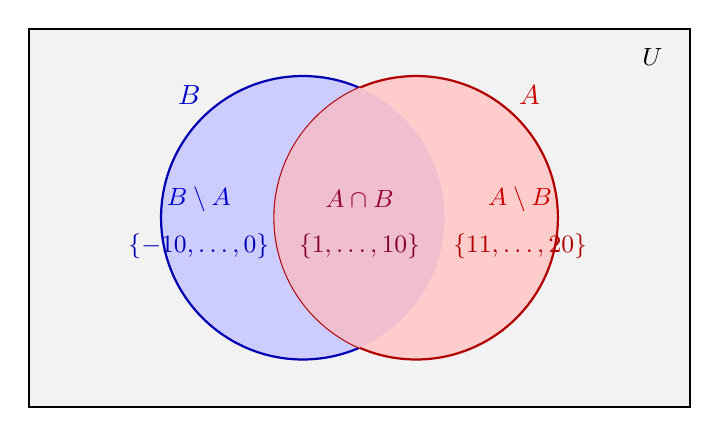
\begin{tikzpicture}[scale=1.2]

  % Universe box
  \fill[gray!10] (-3.5, -2) rectangle (3.5, 2);
  \draw[thick] (-3.5, -2) rectangle (3.5, 2);
  \node[font=\small] at (3.1, 1.7) {$U$};

  % B circle (left)
  \fill[blue!20] (-0.6, 0) circle (1.5cm);
  \draw[thick, blue!70!black] (-0.6, 0) circle (1.5cm);

  % A circle (right)
  \fill[red!20] (0.6, 0) circle (1.5cm);
  \draw[thick, red!70!black] (0.6, 0) circle (1.5cm);

  % Intersection fill
  \begin{scope}
    \clip (-0.6, 0) circle (1.5cm);
    \fill[purple!25] (0.6, 0) circle (1.5cm);
  \end{scope}

  % Labels
  \node[blue!80!black, font=\bfseries] at (-1.8, 1.3) {$B$};
  \node[red!80!black,  font=\bfseries] at ( 1.8, 1.3) {$A$};

  % A setminus B — red only region
  \node[red!80!black,    font=\small] at (1.7,  0.2) {$A \setminus B$};
  \node[red!70!black,    font=\small] at (1.7, -0.3) {$\{11, \ldots, 20\}$};

  % Intersection
  \node[purple!80!black, font=\small] at (0,    0.2) {$A \cap B$};
  \node[purple!70!black, font=\small] at (0,   -0.3) {$\{1, \ldots, 10\}$};

  % B only region
  \node[blue!80!black,   font=\small] at (-1.7,  0.2) {$B \setminus A$};
  \node[blue!70!black,   font=\small] at (-1.7, -0.3) {$\{-10, \ldots, 0\}$};

\end{tikzpicture}
\end{center}
Consider the above venn diagram. $A \setminus B$ is the crescent-shaped bit that opens to the left, shaded in the light red. Note that this operation is cleaner with subsets. For example, consider the subset $C = A \cap B$, $C \subset A$ and $C \subset B$. We have that first,
\[
A \setminus B = A \setminus C ~~\text{  and  }~~ B \setminus A = B \setminus C
\]
and now, the act of excluding objects is much simpler since we do not have to search in $B$ or $A$, respectively, for $A \cap B$ and exclude those objects, since we know that all elements in the set $C$ are in $A$ and $B$. We do not need to search for the overlap if we are "subtracting" a subset since the subset is the overlap. Most times, you will see this "division"/"subtraction" operator be used between sets and subsets, but keep in mind that $A \setminus B$ is valid even thought $B \not\subset A$: we just need to search for $A \cap B$. 

Furthermore, for one final note, let us consider sets that are not defined with the curly braces $\{ \}$. Sometimes, we may define a set by $[1, 5]$. The exact contents of this set will often vary. If we are discussing real numbers, say some real number $r \in [1, 5]$, the set $[1, 5]$ includes all real numbers between 1 and 5, including 1 and 5 themselves. However, if we are discussing some integer $i \in [1, 5]$, then 
\[
i \in \{ 1, 2, 3, 4, 5 \}
\]
and thus 
\[
[1, 5] = \{ 1, 2, 3, 4, 5 \}
\]
when we are discussing integers. It is important that when you see such definitions you consider the universe set - is it real numbers, integers, perhaps even complex numbers - since the definition of sets defined without curly braces will differ based on the context.

Furthermore, let us not a key distinction. Parentheses $()$ are used to denote that the endpoints are not included. For example,
\[
r \in (1, 3) \subset \mathbb{R}
\]
denotes all real numbers between 1 and 3 NOT including either 1 or 3. However,
\[
r \in (1, 3] \subset \mathbb{R}
\]
denotes all real numbers between 1 and 3 not including 1 but does include 3. The same applied for integers, where parenthesis denote exclusion while square brackets denote inclusion. For example,
\[
z \in (1, 3] \subset \mathbb{Z}
\]
denotes that $z \in \{ 2, 3\}$. In this way, sets can often be defined. Note one key rule, though. For sets that are infinitely large, i.e.
\[
r \in (1, \infty) \subset \mathbb{R}
\]
we ALWAYS use a parenthesis on the size of $\pm \infty$ as convention, since a number cannot equal infinity. This same means of set definition via parenthesis and brackets can also be extended to definition via greater-than or less-than signs. For example, $r \in (1, 3] \subset \mathbb{R}$ may be defined as 
\[
1 < r \leq 3
\]
where $r$ is a real number. Integers can also be defined similarly. In these types of definitions, parentheses correspond to $<$ or $>$ (depending on the direction; $3 \geq r > 1$ is also valid but looks a bit weird...), while square brackets correspond to $\leq$ or $\geq$. Similar rules apply with $\pm \infty$, though we typically prefer to use parenthesis-bracket definition for sets with endpoints at an infinity (positive and/or negative) rather than inequalities.

For now, this is a good introduction to sets that you will use throughout your math journey without too much detail for the beginning. We will return to this in Chapter 6.

\section{Miscellaneous Proof Notation}
We will now divert our attention to some common miscellaneous bits of notation. You may have noticed these being used in the first chapter. Mathematicians are a bit lazy; we have developed so much notation as shorthand, but note that in a proof, any of these can be replaced with words! 

Below are some extra symbols, what they mean, and a simple example of their use. You may know some of these fro Problem 1.2.

\qedsymbol . This box is called a QED box, which itself stands for "quod erat demonstrandum". This is Latin for "which was to be demonstrated" which is just a fancy way of saying "thus it's been proven". We use this notation at the end of proofs to signify that our proof is completed and there is no more content in it. Its use is not necessary, but more, a stylistic/semantic choice for organization or sometimes for tradition. You have seen this being used in Chapter 1, when we proved that the inner quadrilateral is a square.

$\in$. This symbol is used to say that an element is inside of a set, or a member of a set. For example, $1 \in \mathbb{N}$ means one is a member of the set of natural numbers. 

$\forall$. This symbol means "for all". I.e. $\forall x \in \mathbb{Z}$, there exists $y \in {Z}$ such that $x + y = 0$. 

$\exists$. This symbol means "there exists" or sometimes just "exists". I.e. $\forall x \in \mathbb{Z}, \exists y \in \mathbb{Z}$ such that $x + y = 0$. 

$\therefore$ This symbol means therefore, i.e. $a = 1, b = 2 \therefore a+b = 3$

For now, this notation will do. I hope that you are a little more armed with knowledge of the tools needed for proofs, along with knowledge of one of the most basic aspects of mathematics: sets.

\section{Problems}

\begin{problem}
    For sets $A$ and $B$, find a formula for $|A \cup B|$ in terms of the cardinalities of other sets involving $A$ and $B$.
\end{problem}

\begin{problem}
Find $(A \cup B)'$ and $(A \cap B)'$ for arbitrary sets $A$ and $B$ in the same universe. These results are known as De Morgan's Laws. \hints{H78, H14, H25}
\end{problem}

\begin{problem}
   Try to prove that $|\mathbb{N}_0| = |\mathbb{Z}|$. \hints{H64}\hfill $\star$
\end{problem}

\begin{problem}
   Show that any number of sets are pairwise mutually exclusive if and only if the cardinality of their union is the sum of their respective cardinalities. Use a proof without words (or with minimal words). This does not have to be a super formal proof, and do not overthink it!
\end{problem}

\begin{problem}
Consider the statement, given $n$ is an integer: ``If  $n^2$ is a multiple of 3, then $n$ is a multiple of 3.''
\begin{enumerate}
    \item Write the negation of this statement.
    \item Write the contrapositive of this statement.
    \item Write the converse of this statement.
\end{enumerate}
\end{problem}

\begin{problem}
Let $A$ be a finite set with cardinality $|A| = n$. The Power Set of $A$, denoted $\mathcal{P}(A)$, is defined as the set of all possible subsets of $A$. For example, if $A = \{1, 2\}$, then $\mathcal{P}(A) = \{\emptyset, \{1\}, \{2\}, \{1, 2\}\}$. Prove that the cardinality of the power set is always 
\[
|\mathcal{P}(A)| = 2^n
\]
\hints{H71, H57}\hfill $\star$
\end{problem}

\begin{problem}
   Does there exist a set that contains itself? Does there exist a set of all sets that contain themselves? Does there exist a set of all sets that do not contain themselves? \hints{H81}\hfill $\star$
\end{problem}